\section{Организационно-экономический раздел}
\subsection{Введение}
В данной части производится расчёт и обоснование стоимости производства разработанного программного комплекса, выполняющего поставленную задачу.
Исходя из анализа существующих на рынке коммерческих решений, можно сделать вывод о приблизительной стоимости готового ПП --- в среднем цена составляет 30~000 руб за одну бессрочную лицензию.

\subsection{Организация и планирование процесса разработки}
При использовании традиционного подхода, организация и планирование процесса разработки программного продукта или программного комплекса предусматривает выполнение следующих работ:

\begin{itemize}
\item формирование состава выполняемых работ и группировка их по стадиям разработки;
\item расчет трудоемкости выполнения работ;
\item установление профессионального состава и расчет количества исполнителей;
\item определение продолжительности выполнения отдельных этапов разработки;
\item построение календарного графика выполнения разработки;
\end{itemize}

Планирование длительности этапов и содержания проекта осуществляется в соответствии с ЕСПД ГОСТ 34.603-92 и распределяет работы по этапам, как показано в таб.~\ref{tab:econ-stages}

\begin{table}[H]
  \begin{tabu}{|c|c|X[l]|}\hline
    Основные стадии & № & Содержание работы \\\hline
    \multirow{2}{*}{Техническое задание} & 1 & Постановка задачи \\\cline{2-3}
         & 2 & Выбор средств разработки и реализации \\\hline
    \multirow{2}{*}{Эскизный проект} & 3 & Разработка математической модели \\\cline{2-3}
         & 4 & Разработка алгоритмов расчёта задачи \\\hline     
    \multirow{2}{*}{Техно-рабочий проект} & 5 & Реализация алгоритмов расчёта задачи \\\cline{2-3}
         & 6 & Разработка пользовательского интерфейса \\\cline{2-3}            
         & 7 & Реализация пользовательского интерфейса \\\hline
    Внедрение & 8 & Проведение вычислительных экспериментов \\\hline
  \end{tabu}
  \caption{Распределение работ по этапам.}
  \label{tab:econ-stages}
\end{table}

\subsection{Расчёт трудоёмкости выполнения работ}
Трудоемкость разработки программной продукции зависит от ряда
факторов, основными из которых являются следующие:
\begin{itemize}
  \item степень новизны разрабатываемого программного комплекса,
  \item сложность алгоритма его функционирования,
  \item объем используемой информации, вид ее представления и способ обработки,
  \item уровень используемого алгоритмического языка программирования
\end{itemize}

Исходные данные расчета приведены в табл.~\ref{tab:econ-init}.

\begin{table}[H]
  \begin{tabu}{|X[l]|>{\centering}m{1.5cm}|X[l]|}\hline
    Функциональное назначение ПП & & Задачи расчётного характера \\\hline
    Алгоритм разработки ПП & 2в &  \\\hline
    Группа новизны & В & Разработка программной продукции, имеющей аналоги \\\hline
    Степень сложности & 1-я группа & Программная продукция, реализующая оптимизационные и моделирующие алгоритмы \\\hline
	По виду представления исходной информации & Группа 12 & Форматный контроль информации. \\\hline
  \end{tabu}
  \caption{Исходные данные}
  \label{tab:econ-init}
\end{table}

Трудоемкость разработки программной продукции $\tau_{ПП}$ может быть определена как сумма величин трудоемкости выполнения отдельных стадий разработки ПП из выражения:

\begin{equation}
	\tau_{ПП} = \tau_{ТЗ} + \tau_{ЭП} + \tau_{ТП} + \tau_{HG} + \tau_{В} 
\end{equation}

где 
\begin{itemize}
  \item $\tau_{ТЗ}$ - трудоемкость разработки технического задания на создание ПП;
  \item $\tau_{ЭП}$ - трудоемкость разработки эскизного проекта ПП;
  \item $\tau_{ТП}$ - трудоемкость разработки технического проекта ПП;
  \item $\tau_{HG}$ - трудоемкость разработки рабочего проекта ПП;
  \item $\tau_{В}$ - трудоемкость внедрения разработанного ПП.
\end{itemize}

Трудоемкость разработки технического задания рассчитывается по формуле:
\begin{equation}
	\tau_{ТЗ} = Т_{ЗРЗ} + Т_{ЗРП}
\end{equation}
где 
\begin{itemize}
  \item $Т_{ЗРЗ}$ - затраты времени разработчика постановки задач на разработку ТЗ, чел. дни;
  \item $Т_{ЗРП}$ - затраты времени разработчика программного обеспечения на разработку ТЗ, чел. дни.
\end{itemize}

В расчёте участвуют следующие коэффициенты:
\begin{itemize}
  \item $t_З = 20$ – норма времени на разработку ТЗ на программный продукт в зависимости от функционального назначения и степени новизны разрабатываемого ПП, чел. дни;
  \item $K_{ЗРЗ} = 0.65$ - коэффициент, учитывающий удельный вес трудоемкости работ, выполняемых разработчиком постановки на стадии ТЗ;
  \item $K_{ЗРП} = 0.35$ - коэффициент, учитывающий удельный вес трудоемкости работ, выполняемых разработчиком программного обеспечения на стадии ТЗ.
\end{itemize}

Тогда
\begin{equation}
	\tau_{ТЗ} = 20 (0.65 + 0.35) = 20 \text{ [чел. дни]}
\end{equation}

Аналогично рассчитывается трудоёмкость эскизного проекта ПП $\tau_{ЭП}$:
\begin{equation}
	\tau_{ЭП} = t_{ЭП} (К_{ЭРЗ} + К_{ЭРП}) = 20 (0.75 + 0.25) = 20 \text{ [чел. дни]}
\end{equation}

Трудоемкость разработки технического проекта $\tau_{ТП}$ зависит от функционального назначения ПП, количества разновидностей форм входной и выходной информации и определяется как сумма времени, затраченного разработчиком постановки задач и разработчиком программного обеспечения, т.е.
\begin{gather*}
	\tau_{ТП} = (t_{ТРЗ} + t_{ТРП}) К_В К_р \\
	К_В = (К_П n_П + К_{НС} n_{НС} + К_Б n_Б) / (n_П + n_{НС} + n_Б)
\end{gather*}

где 
\begin{itemize}
  \item $t_{ТРЗ} = 37, t_{ТРП} = 23$ - норма времени, затрачиваемого на разработку технического проекта разработчиком постановки задач и разработчиком ПП соответственно, чел.-дни
  \item $К_Р = 1,26$ - коэффициент учета режима обработки информации
  \item $К_П = 1, К_НС = 0,72, К_Б = 2.18$ - значения коэффициентов учета вида используемой информации для переменной, нормативно-справочной информации и баз данных соответственно
  \item $n_П = 6, n_НС = 4, n_Б = 0$ - значения коэффициентов учета вида используемой информации для переменной, нормативно-справочной информации и баз данных соответственно
\end{itemize}
Тогда 
\begin{gather*}
	\tau_{ТП} = (37 + 23) (1 \cdot 6 + 0.72 \cdot 4 + 2.18 \cdot 0) / (6 + 4 + 0) \cdot 1.26 = 67 \text{ [чел. дни]}
\end{gather*}

Трудоемкость разработки рабочего проекта $\tau_{РП}$ зависит от
функционального назначения ПП, количества разновидностей форм входной
и выходной информации, сложности алгоритма функционирования,
сложности контроля информации, степени использования готовых
программных модулей, уровня алгоритмического языка программирования и
определяется по формуле:
\begin{gather*}
  \tau_{РП} = К_к К_р К_Я К_З К_{ИА} (t_{РРЗ} + t_{РРП})\\
  К_{ИА} = (К_П' n_П + К_{НС}' n_{НС} + К_Б' n_Б) / (n_П + n_{НС} + n_Б)
\end{gather*}
где
\begin{itemize}
  \item $t_{РРЗ} = 102, t_{РРП} = 348$ - норма времени, затраченного на разработку РП на алгоритмическом языке высокого уровня разработчиком постановки задач и разработчиком программного обеспечения соответственно, чел. дни.
  \item $K_К = 1$ – коэффициент учета сложности контроля информации;
  \item $К_Р = 1.32$ - коэффициент учета режима обработки информации
  \item $K_Я = 1$ – коэффициент учета уровня используемого алгоритмического языка программирования;
  \item $K_З = 0.8$ – коэффициент учета степени использования готовых программных модулей;
  \item $K_{ИА}$ – коэффициент учета вида используемой информации и сложности алгоритма ПП;
  \item $К_П' = 1.20, К_НС' = 0.65, К_Б' = 0.54$ - значения коэффициентов учета сложности алгоритма ПП и вида используемой информации для переменной, нормативно-справочной информации и баз данных соответственно.
\end{itemize}
Тогда
\begin{gather*}
  К_{ИА} = 6 \cdot 1.20 + 4 \cdot 0.65 / (4 + 6) = 0.98 \\
  \tau_{РП} = 1 \cdot 1.32 \cdot 1 \cdot 0.8 \cdot 0.98 \cdot(102 + 348) = 466 \text{ [чел. дни]}
\end{gather*}

Так как при разработке ПП стадии «Технический проект» и «Рабочий
проект» объединены в стадию «Техно-рабочий проект», то трудоемкость ее
выполнения $\tau_{ТРП}$ определяется по формуле:
\begin{gather*}
  \tau_{ТРП} = 0.85 \tau_{ТП} + \tau_{РП} = 0.85 \cdot 67 + 466 = 523 \text{ [чел. дни]}
\end{gather*}

Трудоемкость выполнения стадии внедрения $\tau_{В}$ может быть рассчитана по формуле:
\begin{gather*}
  \tau_{В} = К_к К_р К_З (t_{ВРЗ} + t_{ВРП}) = 1 \cdot 1.32 \cdot 0.8 (30 + 68) = 103 \text{ [чел. дни]}
\end{gather*}

Трудоемкости по этапам разработки проекта представлены в таблице~\ref{tab:econ-trud}.

\begin{table}[H]
  \begin{tabu}{|X[c]|X[c]|}\hline
    Этап & Трудоёмкость этапа, [чел. дни] \\\hline  
    ТЗ & 20 \\\hline  
    ЭП & 20 \\\hline  
    ТРП & 533 \\\hline  
    В & 103 \\\hline      
    Итого & 676 \\\hline        
  \end{tabu}
  \caption{Трудоемкости по стадиям разработки проекта}
  \label{tab:econ-trud}
\end{table}

Средняя численность исполнителей при реализации проекта разработки и внедрения ПО определяется соотношением $N = \frac{Q_p}{F}$, 
где
\begin{itemize}
  \item $Q_p = \tau \cdot t_p$ - затраты труда на выполнение проекта (разработка и внедрение ПО),
  \item $F = T \cdot F_M$ - фонд рабочего времени;
  \item $Т$ - время выполнения проекта в месяцах. T = 5 мес.;
  \item $F_M$ - фонд времени в текущем месяце, который рассчитывается из учета общества числа дней в году, числа выходных и праздничных дней и определяется соотношением $F_М = \frac{t_p (D_k - D_B - D_П)}{12}$;
  \item $t_p$ - продолжительность рабочего дня;
  \item $D_K$ - общее число дней в году;
  \item $D_B$ - число выходных дней в году;
  \item $D_П$ - число праздничных дней в году.
\end{itemize}

Тогда 
\begin{gather*}
  F = 5 \cdot 8 (365 - 103 - 13) / 12 = 830\\
  N = 676 \cdot 8 / 830 = 7 \text{ - число исполнителей проекта.}
\end{gather*}

\subsection{Календарный план-график}
Планирование и контроль хода выполнения разработки проводится по календарному графику выполнения работ. Планирование процесса разработки и календарный ленточный план представлены в таб. \ref{tab:econ-plan} и рис. \ref{tab:econ-lent} соответственно.

\begin{table}[H]
  \begin{tabu} to \textwidth {|m{2cm}|m{1,5cm}|m{4cm}|m{3cm}|X|}\hline
    Стадия & $\tau$ & Должность исполнителя & Распределение трудоемкости & Числ-ть \\\hline
    ТЗ & 20 & \shortstack{Ведущий инженер\\Программист} & \shortstack{15(75 \%)\\5} & \shortstack{1\\1} \\\hline  
    ЭП & 20 & \shortstack{Ведущий инженер\\Программист} & \shortstack{12(60 \%)\\8} & \shortstack{1\\1} \\\hline  
    ТРП & 533 & \shortstack{Ведущий инженер\\Программист} & \shortstack{71\\6 \times 76} & \shortstack{1\\6} \\\hline  
    В & 103 & \shortstack{Ведущий инженер\\Программист} & \shortstack{13\\3 \times 30} & \shortstack{1\\3} \\\hline      
    Итого & 676 & & & 7 \\\hline  
  \end{tabu}
  \caption{Планирование процесса разработки.}
  \label{tab:econ-plan}
\end{table}

\begin{figure}[H]
  \centering
  \includegraphics[width=.5\textwidth]{img/timeplan}
  \caption{Календарный ленточный план работ.}
  \label{tab:econ-lent}
\end{figure}

Вывод: при распараллеливании работы ведущего инженера и
программистов можно добиться сокращения срока разработки и внедрения
программного продукта с 676 дней до 133 дней, т. е. в 5.08 раза по сравнению
со временем разработки одним человеком.

В таб. \ref{tab:econ-salary} приведены затраты на заработную плату и отчисления
на социальное страхование в пенсионный фонд, фонд занятости и фонд
обязательного медицинского страхования (30\%). Для всех исполнителей
предполагается оклад в размере 20000 рублей в месяц.

\begin{table}[H]
  \centering
  {
  \begin{tabu} to \textwidth {||c|*{3}{|X|X|X|}|c||}\hline
   & \multicolumn{3}{c||}{Г.И.} & \multicolumn{3}{c||}{П1} & \multicolumn{3}{c||}{П2..6} & Всего \\\hline
   Мес & Р.Д. & ЗП & ЕСН & Р.Д. & ЗП & ЕСН & Р.Д. & ЗП & ЕСН & \\\hline
   1 & 21 & 20 & 6 & 10 & 9.52 & 2.86 &  &  &  & 38.38 \\\hline
   2 & 21 & 20 & 6 & 11 & 10.48 & 3.14 & 7 & 6,67 & 2 & 48.29 \\\hline
   3 & 21 & 20 & 6 & 21 & 20 & 6 & 21 & 20 & 6 & 78.00 \\\hline
   4 & 21 & 20 & 6 & 21 & 20 & 6 & 21 & 20 & 6 & 78.00 \\\hline
   5 & 21 & 20 & 6 & 21 & 20 & 6 & 21 & 20 & 6 & 78.00 \\\hline
   6 & 20 & 19.05 & 5.71 & 21 & 20 & 6 & 21 & 20 & 6 & 76.76 \\\hline
   \multicolumn{10}{||l||}{Итого:}  & 320.67 \\\hline   
  \end{tabu}}
  \caption{Затраты на зарплату и отчисления на социальное страхование, тыс.руб.}
  \label{tab:econ-salary}
\end{table}

Расходы на материалы, необходимые для разработки программной
продукции, указаны в таблице \ref{tab:econ-materials}.

\begin{table}[H]
  \centering
  \begin{tabu} to \textwidth {|c|c|X|X|X|}\hline
    Наименование & Единица & К-во & Цена/ед. & Сумма \\
    материала & измерения & & (руб.)& (руб.) \\\hline
    Бумага А4 & Пачка 500 листов & 2 & 200 & 400\\\hline
    Картридж Canon IP5200 & Картридж, 10мл & 5 & 300 & 1500\\\hline
    \multicolumn{4}{|l|}{Итого:} & 1900 \\\hline
  \end{tabu}
  \caption{Затраты на материалы.}
  \label{tab:econ-materials}
\end{table}

В работе над проектом используется специальное оборудование –
персональные электронно-вычислительные машины (ПЭВМ) в количестве 14
шт. Стоимость одной ПЭВМ составляет 20~000 рублей. Согласно нормативным документам, срок амортизации ПЭВМ составляет 3 года, что определяет месячную норму амортизации K = 2.7\%.

Тогда за 5 месяцев работы расходы на амортизацию составят $20~000 \cdot 14 \cdot 0.027 \cdot 5 = 37~800 \text{руб.}$

Общие затраты на разработку ПП составят:

\begin{gather*}
  C = 320~670 + 1~900 + 37~800 = 360~370 \text{ руб.}
\end{gather*}

\subsection{Расчёт стоимости программного продукта}
Цена ПП рассчитывается по формуле:
\begin{gather*}
  Ц = С + Пр\\
  Пр = \frac{(С-С_м)р_н}{100 \%}
\end{gather*}
где
\begin{itemize}  
 \item $С$ - затраты на разработку ПП\\
 \item $С_м$ - материальные затраты, руб./изд\\
 \item $Пр$ - желаемая прибыль\\ 
 \item $р_н$ - норматив рентабельности, принимаемый разработчиком\\  
\end{itemize}

Тогда
\begin{gather*}
  Ц = 360~370 + (360~370 - 37~800 - 1~900) \cdot 0.25 = 440~538 \text{ руб.}
\end{gather*}

\subsection{Расчет экономической эффективности}

Основными показателями экономической эффективности является
чистый дисконтированный доход (ЧДД) и срок окупаемости вложенных
средств.

Чистый дисконтированный доход определяется по формуле:
\begin{gather*}
  ЧДД = sum_{t=0}^T (R_t - З_t) \frac{1}{(1 + E)^t}
\end{gather*}
где
\begin{itemize}
  \item $Т$ - горизонт расчета по месяцам;
  \item $t$ - период расчета;
  \item $R_t$ - доход за текущий месяц;
  \item $З_t$ - затраты за текущий месяц;
  \item $E$ - приемлемая для инвестора норма прибыли на вложенный капитал.
\end{itemize}

Коэффициент E установим равным ставке рефинансирования ЦБ РФ – 8.25\%
годовых (или 0.66\% в месяц). В виду особенности разрабатываемого продукта
он может быть продан лишь однократно.
Коэффициент дисконтирования равен 1/(1 + Е) = 0.99.

В таб. \ref{tab:econ-chdd} приведен расчет ЧДД по месяцам работы над проектом.

График ЧДД приведён на рис.~\ref{fig:econ-chdd}.
\begin{table}[H]
  \centering
  \begin{tabu} to \textwidth {|c|X|X|X|X|}\hline
    Месяц & Тек. Затр. & Общ. Затр. & Тек.доход & ЧДД \\\hline
    1 & 46130,95 & 46130,95 & 0,00 & -45669,64 \\\hline
    2 & 56035,71 & 102166,67 & 0,00 & -84815,30 \\\hline
    3 & 85750,00 & 187916,67 & 0,00 & -142790,67 \\\hline
    4 & 85750,00 & 273666,67 & 0,00 & -208511,45 \\\hline
    5 & 85750,00 & 359416,67 & 0,00 & -314784,59 \\\hline
    6 & 84511,90 & 443928,57 & 440538,00 & 20406,92 \\\hline
  \end{tabu}
  \label{tab:econ-chdd}
  \caption{Расчёт ЧДД.}
\end{table}

\begin{figure}[H]
  \centering
  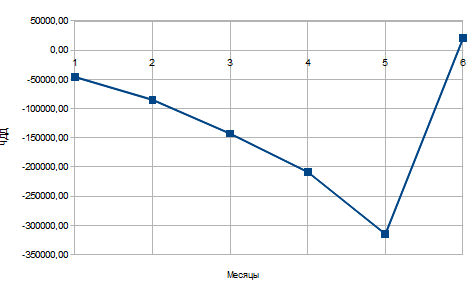
\includegraphics[width=.9\textwidth]{img/chddplot}
  \caption{График изменения чистого дисконтированного дохода.}
  \label{fig:econ-chdd}
\end{figure}

\subsection{Вывод}
Исходя из расчётов, можно сделать вывод о том, что проект окажется рентабельным, а затраты на его выполнение
окупятся. Итоковый ЧДД равен 20~406.92 рублей. Срок реализации проекта составляет 6 месяцев.